% Options for packages loaded elsewhere
\PassOptionsToPackage{unicode}{hyperref}
\PassOptionsToPackage{hyphens}{url}
%
\documentclass[
  9pt,
  ignorenonframetext,
]{beamer}
\usepackage{pgfpages}
\setbeamertemplate{caption}[numbered]
\setbeamertemplate{caption label separator}{: }
\setbeamercolor{caption name}{fg=normal text.fg}
\beamertemplatenavigationsymbolsempty
% Prevent slide breaks in the middle of a paragraph
\widowpenalties 1 10000
\raggedbottom
\setbeamertemplate{part page}{
  \centering
  \begin{beamercolorbox}[sep=16pt,center]{part title}
    \usebeamerfont{part title}\insertpart\par
  \end{beamercolorbox}
}
\setbeamertemplate{section page}{
  \centering
  \begin{beamercolorbox}[sep=12pt,center]{part title}
    \usebeamerfont{section title}\insertsection\par
  \end{beamercolorbox}
}
\setbeamertemplate{subsection page}{
  \centering
  \begin{beamercolorbox}[sep=8pt,center]{part title}
    \usebeamerfont{subsection title}\insertsubsection\par
  \end{beamercolorbox}
}
\AtBeginPart{
  \frame{\partpage}
}
\AtBeginSection{
  \ifbibliography
  \else
    \frame{\sectionpage}
  \fi
}
\AtBeginSubsection{
  \frame{\subsectionpage}
}
\usepackage{lmodern}
\usepackage{amsmath}
\usepackage{ifxetex,ifluatex}
\ifnum 0\ifxetex 1\fi\ifluatex 1\fi=0 % if pdftex
  \usepackage[T1]{fontenc}
  \usepackage[utf8]{inputenc}
  \usepackage{textcomp} % provide euro and other symbols
  \usepackage{amssymb}
\else % if luatex or xetex
  \usepackage{unicode-math}
  \defaultfontfeatures{Scale=MatchLowercase}
  \defaultfontfeatures[\rmfamily]{Ligatures=TeX,Scale=1}
\fi
\usetheme[]{Goettingen}
\usecolortheme{rose}
% Use upquote if available, for straight quotes in verbatim environments
\IfFileExists{upquote.sty}{\usepackage{upquote}}{}
\IfFileExists{microtype.sty}{% use microtype if available
  \usepackage[]{microtype}
  \UseMicrotypeSet[protrusion]{basicmath} % disable protrusion for tt fonts
}{}
\makeatletter
\@ifundefined{KOMAClassName}{% if non-KOMA class
  \IfFileExists{parskip.sty}{%
    \usepackage{parskip}
  }{% else
    \setlength{\parindent}{0pt}
    \setlength{\parskip}{6pt plus 2pt minus 1pt}}
}{% if KOMA class
  \KOMAoptions{parskip=half}}
\makeatother
\usepackage{xcolor}
\IfFileExists{xurl.sty}{\usepackage{xurl}}{} % add URL line breaks if available
\IfFileExists{bookmark.sty}{\usepackage{bookmark}}{\usepackage{hyperref}}
\hypersetup{
  pdftitle={BIOS6643 Longitudinal},
  pdfauthor={EJC},
  hidelinks,
  pdfcreator={LaTeX via pandoc}}
\urlstyle{same} % disable monospaced font for URLs
\newif\ifbibliography
\usepackage{longtable,booktabs}
\usepackage{calc} % for calculating minipage widths
\usepackage{caption}
% Make caption package work with longtable
\makeatletter
\def\fnum@table{\tablename~\thetable}
\makeatother
\setlength{\emergencystretch}{3em} % prevent overfull lines
\providecommand{\tightlist}{%
  \setlength{\itemsep}{0pt}\setlength{\parskip}{0pt}}
\setcounter{secnumdepth}{-\maxdimen} % remove section numbering
\AtBeginSubsection{}
\AtBeginSection{}
\ifluatex
  \usepackage{selnolig}  % disable illegal ligatures
\fi

\title{BIOS6643 Longitudinal}
\subtitle{L10 Nesting and Cross I}
\author{EJC}
\date{}
\institute{Department of Biostatistics \& Informatics}

\begin{document}
\frame{\titlepage}

\begin{frame}[allowframebreaks]
  \tableofcontents[hideallsubsections]
\end{frame}
\hypertarget{nesting-and-cross}{%
\section{Nesting and Cross}\label{nesting-and-cross}}

\begin{frame}{Topics for this lecture}
\protect\hypertarget{topics-for-this-lecture}{}
\begin{itemize}
\tightlist
\item
  Nesting and crossing
\end{itemize}

\vspace{\baselineskip}

\begin{itemize}
\item
  \textbf{Associated reading: Course notes}

  \begin{itemize}
  \item
    `Nesting and crossing' section in LMM chapter
  \item
    Hedeker, Ch. 13 (for hierarchical models)
  \end{itemize}
\end{itemize}
\end{frame}

\hypertarget{nested-versus-crossed-factors}{%
\section{Nested versus crossed
factors}\label{nested-versus-crossed-factors}}

\begin{frame}{Definitions}
\protect\hypertarget{definitions}{}
\begin{itemize}
\item
  The term \textbf{nesting} can be applied to many things, including
  design structures, treatment structures, factors, data or models.
\item
  Factors A and B are \textbf{crossed} if every level of A appears with
  every level of B. Such is the case for a 2-factor factorial treatment
  structure in a completely randomized design. Example: Myostatin
  experiment.
\item
  Factors are \textbf{nested} when the levels of one factor occur with
  only one level of another factor. For example, consider a experiment
  designed to determine the effect of school and instructor on
  standardized test scores of kids in elementary schools, where each
  school has a unique set of teachers.
\item
  Factors may be crossed even when units are nested.
\item
  For example, if you have Day (1, 2, 3, \ldots) and Time of Day
  (morning, noon, evening), then units for Time of Day appear to be
  nested within Day.
\item
  However, if `morning', `noon' and `evening' have consistent meanings
  across days, then Day and Time of Day can be considered crossed
  factors.
\end{itemize}
\end{frame}

\begin{frame}{Examples:}
\protect\hypertarget{examples}{}
\begin{block}{Crossed (e.g., Myostatin data)}
\protect\hypertarget{crossed-e.g.-myostatin-data}{}
\begin{longtable}[]{@{}cccc@{}}
\toprule
& Time1 & Time2 & Time3\tabularnewline
\midrule
\endhead
Group A & X & X & X\tabularnewline
Group B & X & X & X\tabularnewline
\bottomrule
\end{longtable}
\end{block}

\begin{block}{Nested (e.g., standardized test data)}
\protect\hypertarget{nested-e.g.-standardized-test-data}{}
\begin{longtable}[]{@{}cccccc@{}}
\toprule
& Teacher1 & Teacher2 & Teacher3 & Teacher4 & Teacher5\tabularnewline
\midrule
\endhead
School A & X & X & & &\tabularnewline
School B & & & X & X &\tabularnewline
School C & & & & & X\tabularnewline
\bottomrule
\end{longtable}
\end{block}
\end{frame}

\hypertarget{nesting}{%
\section{Nesting}\label{nesting}}

\begin{frame}{Notation for nesting:}
\protect\hypertarget{notation-for-nesting}{}
\begin{itemize}
\item
  On factors: for B nested within A, you may see \textbf{B (A)} (e.g.,
  SAS uses this).
\item
  On indices: if \(i\) and \(j\) are indices for factors A and B,
  respectively, and B is nested within A, then an effect in the model
  may be denoted as \(\beta_{(j(i))}\).
\item
  In SAS, when you specify B(A), you are telling SAS that B is nested
  within A. Due to this, levels of B are unique within A; you have to
  consider the levels of B separate for each level of A, just like an
  interaction. The code below shows equivalency of B(A) and
  \(B \times A\).
\end{itemize}
\end{frame}

\begin{frame}{Nesting and interaction}
\protect\hypertarget{nesting-and-interaction}{}
\begin{itemize}
\tightlist
\item
  The data set below involves measurements taken within days (e.g.,
  morning, noon, evening), for 3 different days. We would consider
  factors A and B crossed if the levels `morning', `noon' and `evening'
  mean the same thing across days, and we would consider B nested within
  A if the levels of B could not be considered the same -- e.g., if
  times of measurement varied across days. The data and partial output
  follows.
\end{itemize}

\begin{center}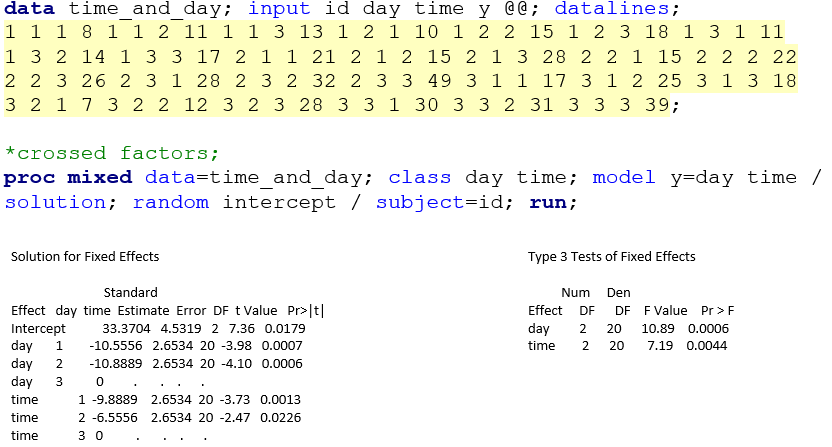
\includegraphics[width=1\linewidth]{figs_L10/f1} \end{center}
\end{frame}

\begin{frame}{}
\protect\hypertarget{section}{}
\begin{itemize}
\tightlist
\item
  Estimates for specific \(time \times day\) combinations can be
  determined from the factor `marginal' estimates (plus the intercept).
  `Marginal'=main effect in this case.
\end{itemize}

\begin{center}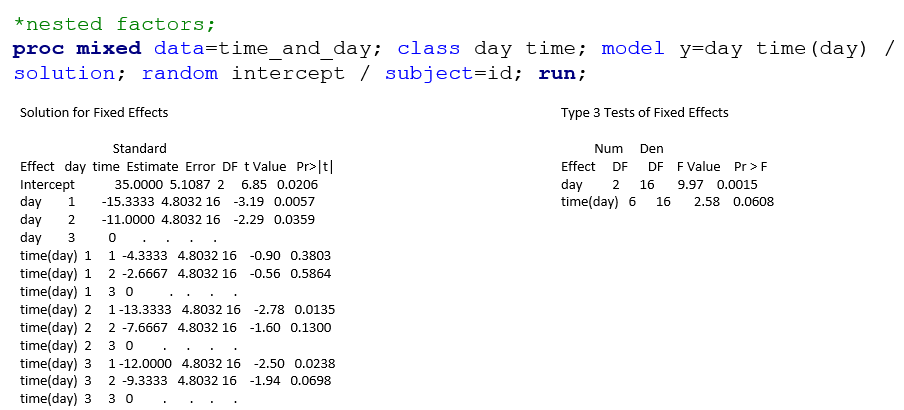
\includegraphics[width=1\linewidth]{figs_L10/f2} \end{center}

\begin{itemize}
\tightlist
\item
  Using \(time \times day\) in place of time(day) will yield the same
  SAS output. In this case, each \(time \times day\) combination has a
  unique estimate such that `marginal' factor estimates cannot be used
  to obtain them.
\end{itemize}
\end{frame}

\begin{frame}{}
\protect\hypertarget{section-1}{}
\begin{itemize}
\item
  Determining whether factors are crossed or nested should not be based
  on model fit; rather, it should be based on the design of the
  experiment or study. But in some cases, there may be a fine line
  between whether factors are nested or crossed.
\item
  In the example above, we said that factors are crossed if the levels
  of time meant the same thing across days. The question is, how close
  in actual time do the measurements need to be to be considered `the
  same'?

  For the crossed design, you could also include \(time \times day\) in
  the model. The test for \(time \times day\) will not be the same as
  for time(day) (or \(time \times day\)) in the nested models above.
  But, the LSMEANS estimates for \(time \times day\) combinations will
  be the same between the `full' and nested models.
\end{itemize}
\end{frame}

\begin{frame}{Nested subjects}
\protect\hypertarget{nested-subjects}{}
\begin{itemize}
\item
  Before, we saw the use of the nested notation for subjects within
  groups. This relates to a parallel experiment in which subjects are
  randomly assigned to groups, and remain in those groups throughout the
  experiment. This differs from a crossover experiment. (These will be
  discussed more in the next section.)
\item
  For a parallel study/experiment, the use of ID(GROUP) is important in
  SAS PROC MIXED if the same IDs are used in different groups. When
  using PROC GLM for repeated measures ANOVA, the use of this nested
  variable is important whether or not the IDs are repeated.
\end{itemize}
\end{frame}

\begin{frame}[fragile]{Nested versus crossed random effects}
\protect\hypertarget{nested-versus-crossed-random-effects}{}
\begin{itemize}
\item
  Nesting and crossing apply to random effects as well as fixed effects.
  Consider the standardized test data. If the given teachers and schools
  form a (random) sample from this population, then we can model school
  as one random effect term, and teacher within school {[}or
  teacher(school){]} as another. The random statement in the PROC MIXED
  code would be:

\begin{verbatim}
RANDOM school teacher(school);
\end{verbatim}
\item
  For the psychological scoring data, the first approach was to model
  subject and rater as random effects. Since each rater scored each
  subject, then the random effects were crossed:

\begin{verbatim}
RANDOM subject rater;
\end{verbatim}
\end{itemize}
\end{frame}

\hypertarget{hierarchical-linear-models}{%
\section{Hierarchical Linear Models}\label{hierarchical-linear-models}}

\begin{frame}{Two-level models}
\protect\hypertarget{two-level-models}{}
\begin{itemize}
\item
  A mixed model with subjects that are observed over time can be
  considered a hierarchical model, where the level 1 model consists of
  the responses over time for subjects (\(Y_{ij}\)), and the level 2
  model consists of subject-specific random effect terms. Specifically,
  considering the random intercept model, we have

  Level 1: \(Y_{ij}=b_{0i}+b_{1i} t_{ij}+\epsilon_{ij}\)

  Level 2: \(b_{0i}=\beta_0+u_{0i};\ b_{1i}=\beta_1\)
\item
  If we desire to have random slopes (for time) in the 2-level model as
  well as random intercepts, then we have

  Level 1: \(Y_{ij}=b_{0i}+b_{1i} t_{ij}+\epsilon_{ij}\)

  Level 2: \(b_{0i}=\beta_0+u_{0i}; \ b_{1i}=\beta_1+u_{1i}\)
\end{itemize}
\end{frame}

\begin{frame}{}
\protect\hypertarget{section-2}{}
\begin{itemize}
\item
  Other types of 2-level models may not involve repeated measures.
\item
  E.g. health care costs for individuals with different health insurance
  providers at one time.

  \begin{itemize}
  \item
    The level 1 model would involve the subjects (\(Y_{ij}\), \(i\)
    denotes provider, \(j\) denotes subject).
  \item
    The level 2 model would involve the providers.
  \item
    Here, subjects are nested within health-care providers, and this
    could be modeled using a random intercept term for provider; subject
    variability will be accounted for with the residual error term. The
    model could be expressed as:
  \end{itemize}

  Level 1: \(Y_{ij}=b_{0i}+\epsilon_{ij}\) (costs for individuals)

  Level 2: \(b_{0i}=\beta_0+u_{0i}\) (random insurance provider effects)
\end{itemize}
\end{frame}

\begin{frame}{}
\protect\hypertarget{section-3}{}
\begin{itemize}
\item
  For the standardized test data, if there is one response per teacher,
  the level 1 model would involve subjects within schools, and the level
  2 model would involve the schools.
\item
  \emph{Applying level terminology to the units}. For the standardized
  test data, the level 1 units involve teachers and level 2 units
  involve schools. For the 3-level HLM with insurance data, the level 1
  units involve the repeated measures over time, the level 2 units would
  be subjects, and level 3 units would be the providers.
\item
  \emph{Distinguishing `nesting' concepts for factors and data}.
  Although we may say that repeated measures are `nested' within
  subjects, it is possible that the factor associated with the repeated
  measures (e.g., time) is crossed with subjects, if there are specific
  measurement times that every subject is observed at. Thus, we need to
  distinguish nesting/crossing of data versus nesting/crossing of
  factors.
\end{itemize}
\end{frame}

\begin{frame}{Three-level models}
\protect\hypertarget{three-level-models}{}
\begin{block}{Examples}
\protect\hypertarget{examples-1}{}
For the insurance provider data, suppose that we have repeated cost
measures for subjects over time. A 3-level hierarchical model could be
developed for these data, where health care costs are denoted as
\(Y_{ijk}\), where i=provider, \(j\)=subject, \(k\)=time.

\begin{itemize}
\item
  The level 1 model involves repeated measures within subjects, the
  level 2 model involves the subjects themselves, and the level 3 model
  involves the health care providers.
\item
  This model may include two random intercept terms, one for provider,
  and one for subject within provider.
\item
  The lowest level (i.e., level 1) of a hierarchical model involves the
  smallest unit of measurement while the highest level involves the
  largest unit of measurement.
\end{itemize}
\end{block}
\end{frame}

\begin{frame}{}
\protect\hypertarget{section-4}{}
\begin{block}{Example 1: Subjects that are obtained from different sites
are monitored over time (perhaps after being assigned to a treatment
group).}
\protect\hypertarget{example-1-subjects-that-are-obtained-from-different-sites-are-monitored-over-time-perhaps-after-being-assigned-to-a-treatment-group.}{}
\begin{itemize}
\item
  This is often called a multi-site experiment or study, which is done
  because it is too difficult for one site alone to get all of the
  subjects for the experiment.
\item
  For example, the sites may be medical and research centers across the
  U.S.
\item
  Here, leve1 1 involves the measures on subjects over time. Level 2
  involves the subjects that are nested within sites, and level 3
  involves the sites. (Of course, measures on subjects are nested within
  subjects!)
\end{itemize}
\end{block}

\begin{block}{Example 2 Children are recruited from schools for a health
study.}
\protect\hypertarget{example-2-children-are-recruited-from-schools-for-a-health-study.}{}
\begin{itemize}
\item
  Children are obtained by selecting them from classrooms within schools
  within the study area.
\item
  The level 1 units involve the children's measurements; the level 2
  units are classrooms and the level 3 units are the schools.
\item
  Note that children are nested within classrooms and classrooms are
  nested within schools.
\item
  We could extend this to 4-level data if repeated measures were taken
  on the children, where the repeated measures within subjects would
  become the level 1 data.
\end{itemize}
\end{block}
\end{frame}

\hypertarget{case-study}{%
\section{Case study}\label{case-study}}

\begin{frame}{Case study: Kunsberg study}
\protect\hypertarget{case-study-kunsberg-study}{}
An EPA-funded study at NJH has involved kids from the Kunsberg School
(at NJH) that have moderate to severe asthma. One of the primary goals
has been to determine how the health of children is associated with air
pollution on a day-to-day basis. A number of variables have been
collected on subjects (demographic, behavioral, and biological) as well
as the environment (air pollution, meteorology) for this ongoing study.

One of the difficulties with the data is that siblings are often
involved in the study. For the 2001-02 school year, there were 48
subjects from 40 families; in 2002-03, there were 57 children from 52
families. In both years, there were never more than 2 kids involved from
the same family.
\end{frame}

\begin{frame}{}
\protect\hypertarget{section-5}{}
One of the key assumptions in our modeling is the `independent subjects'
assumption. In medical research, this assumption is often ignored.
People often fret more about the normality assumption and ignore the
independence assumption, the latter of which can be much more
problematic.

One of the reasons why the independence assumption is violated in
medical research is because random sampling is usually unfeasible.
Participants are often self selected. We can account for the possible
dependency between siblings by including appropriate random terms. We
can fit the model with and without the random terms to determine the
impact of the dependency.
\end{frame}

\begin{frame}{}
\protect\hypertarget{section-6}{}
This can be considered 3-level data, where

\begin{itemize}
\item
  families are the level 3 unit
\item
  children within families are the level 2 unit
\item
  repeated measures within kids are the level 1 unit.
\end{itemize}

For this analysis, LTE4 (a specific biomarker in the body that has been
shown to be associated with inflammation) was fit on the natural log
scale as a function of date (linear time trend), cold (1=yes, 0=no -- a
time varying variable), temperature, pressure and humidity. The goal is
to better understand how LTE4 relates to different variables over time.
{[}Side note: it has already been shown that LTE4 is related to air
pollution. See Rabinovitch, Strand, Gelfand, 2006 AJRCCM article.{]}
\end{frame}

\begin{frame}{The model}
\protect\hypertarget{the-model}{}
We could write \(Y_{ij}\) on the left since an observation is uniquely
identified by subject and date. Here I include it for sake of
completeness.

\(Y_{hij}=\beta_0+\beta_1 date_j+\beta_2 cold_{ij}+\beta_3 temp_j+\beta_4 pressure_j+\beta_5 humidity_j+b_h+b_{(i(h))}+\epsilon_{ij}\)

\(b_h \sim \mathcal N(0,\ \sigma_F^2)\)

\(b_{i(h)} \sim \mathcal N(0,\ \sigma_S^2)\)

\(\epsilon_{ij} \sim \mathcal N(0,\ \sigma_\epsilon^2)\)

\(h\) for family, \(i\) for subject, \(j\) for time.

\(\pmb \epsilon_i \sim \mathcal N(0,\ R_i)\), where \(R_i\) has the
AR(1) form.
\end{frame}

\begin{frame}{SAS code:}
\protect\hypertarget{sas-code}{}
\begin{center}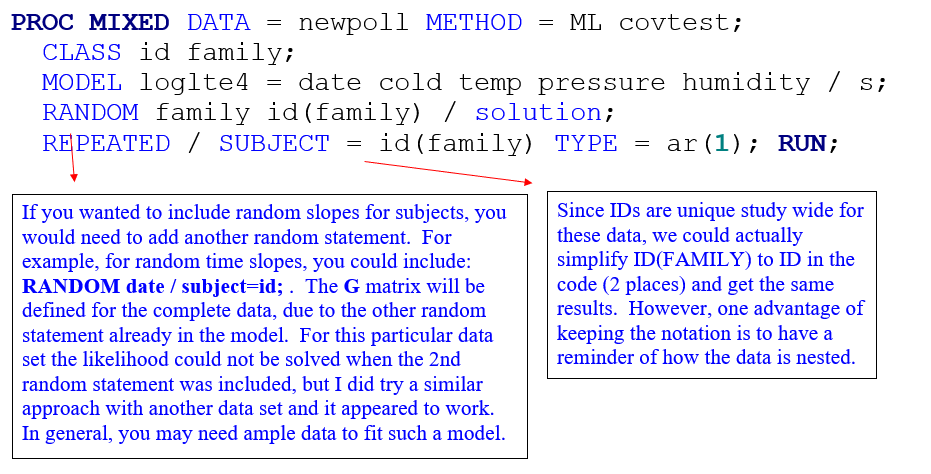
\includegraphics[width=1\linewidth]{figs_L10/f3} \end{center}
\end{frame}

\begin{frame}{Abbreviated output:}
\protect\hypertarget{abbreviated-output}{}
\begin{center}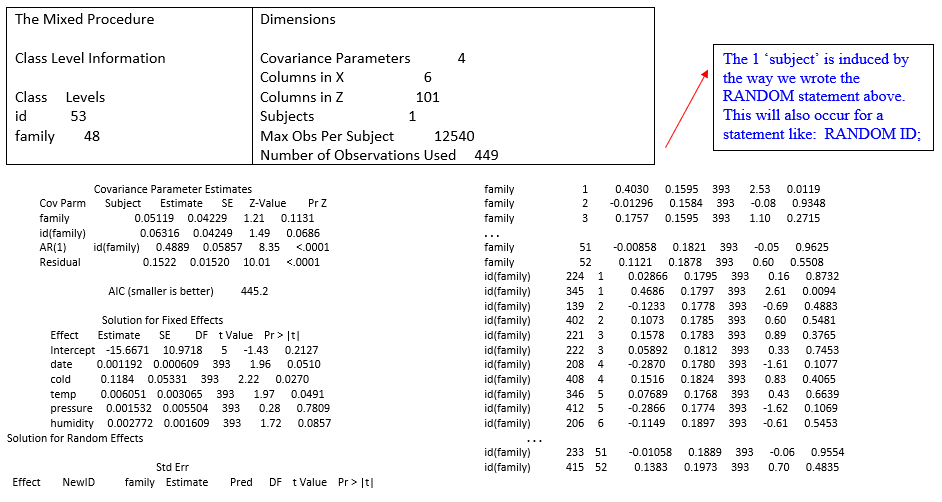
\includegraphics[width=1\linewidth]{figs_L10/f4} \end{center}
\end{frame}

\begin{frame}{Model without family}
\protect\hypertarget{model-without-family}{}
\begin{center}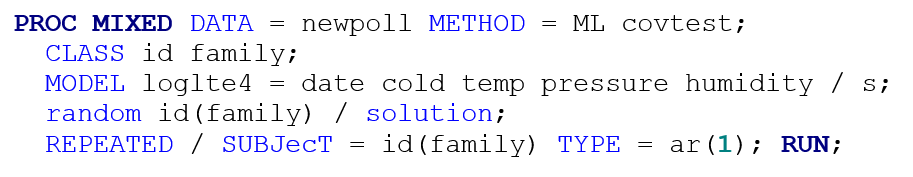
\includegraphics[width=1\linewidth]{figs_L10/f5} \end{center}

\begin{center}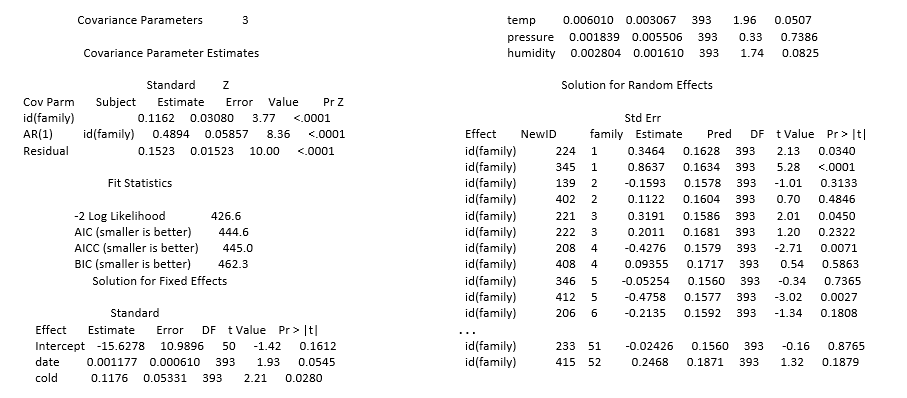
\includegraphics[width=1\linewidth]{figs_L10/f6} \end{center}
\end{frame}

\begin{frame}{Synopsis}
\protect\hypertarget{synopsis}{}
\begin{itemize}
\item
  The estimated variance for families and subjects within families have
  roughly the same order of magnitude. By looking at the 2nd output, we
  can see that the ID(FAMILY) variance then absorbs all of the variance
  that was formerly attributed to the random family effect.
\item
  There is not a dramatic difference in fixed effect estimates for the 2
  approaches. The AICs are comparable, but a bit better without the
  family effect. It is likely that the level of dependency due to
  siblings is not that great since there are few siblings involved.
\item
  Even though removal of the random term for family (and hence not
  accounting for the sibling effect) did not change estimates
  drastically, I would generally warn against ignoring dependent data!
  It would be prudent to at least check for it,
\end{itemize}
\end{frame}

\begin{frame}{}
\protect\hypertarget{section-7}{}
\begin{itemize}
\item
  If relevant, it is also possible to examine nested effects for random
  slopes.

  \begin{itemize}
  \item
    For example, we previously discussed the relationship between
    personal exposure to ambient PM2.5 and actual ambient PM2.5.
  \item
    Subjects have different slopes, based somewhat on the type of
    housing they live in. Thus, it may be expected that subjects that
    live in the same house (i.e., those within the same family) will
    tend to have the same slopes.
  \end{itemize}
\item
  In this case, we may try fitting two random slopes for ambient PM2.5
  to account for this dependency, one for SUBJECT=FAMILY and the other
  for SUBJECT=ID(FAMILY).
\item
  For further details on hierarchical models fit to multi-level data
  (with an emphasis on the use of SAS PROC MIXED), see \textbf{Littell
  et al., SAS System for Mixed Models}.
\end{itemize}
\end{frame}

\end{document}
